\chapter{Introduction}

\begin{figure}[h!]
	\caption{Application Dashboard}
	\label{image:dashboard1}
	\centering
	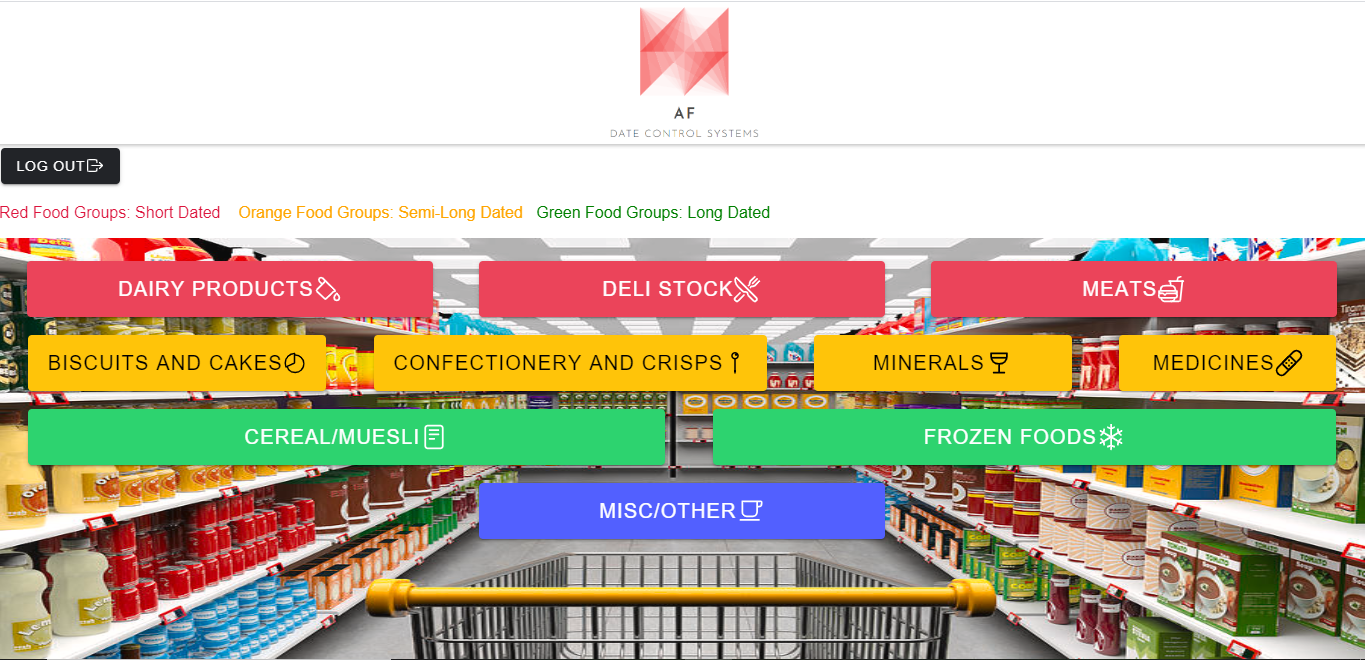
\includegraphics[width=1\textwidth]{images/dashboard.PNG}
\end{figure}

The Final Year Project was a great opportunity for me to culminate what I have learned in the four years of study in the field of software development to produce the project of my choosing. When deciding what to develop for the final year project, I needed to split it up in to many different aspects. The idea, the reasoning and why it would be beneficial for human use and also economically sufficient for the target audience. A decision on technology to use needed to be made also, what programming language to use, pros and cons, what database storage to use to store data applicable to what I was going to develop.  

\begin{figure}[h!]
	\caption{Various Software Languages to choose from.}
	\label{image:progLanguages}
	\centering
	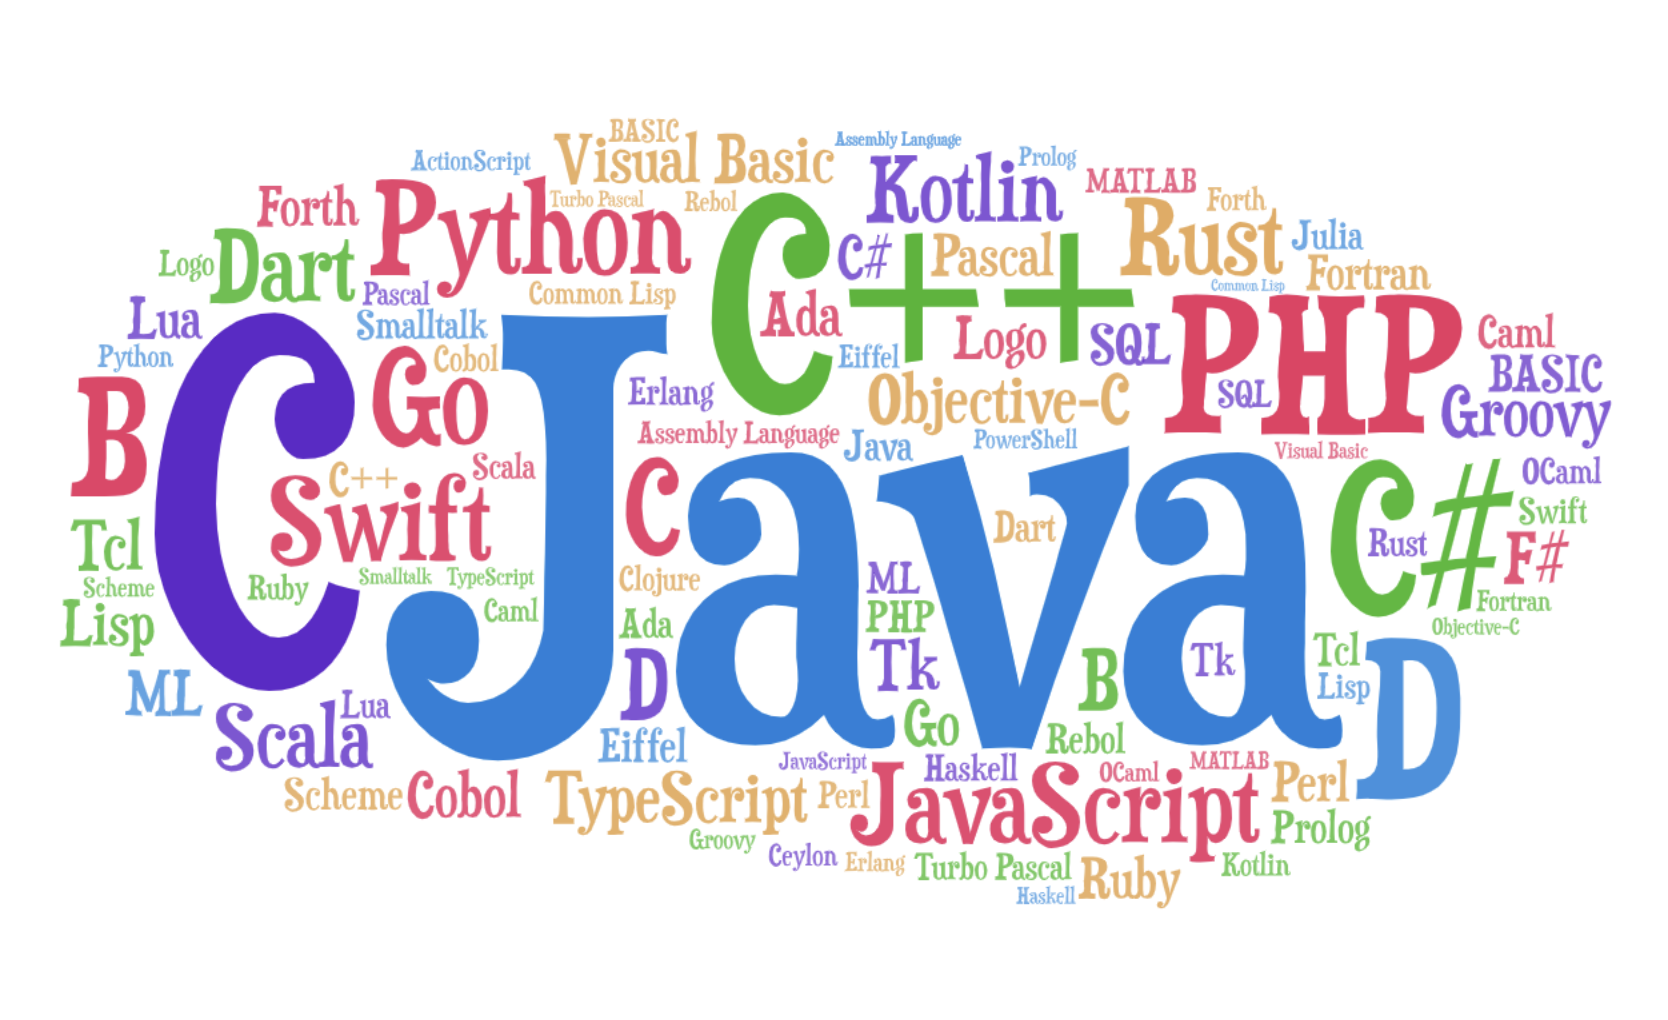
\includegraphics[width=0.8\textwidth]{images/progLanguages.png}
\end{figure}	

\newpage

When deciding on what type of project and application to pursue, I wanted to integrate it into something involved in weekly life. My part time job as a Sales Assistant had a massive influenced in making a decision on what type of project to do. I looked into the everyday operation of the shop, after working there for just under five years the experience was there in knowing the day to day operations of the store. I looked at different ways I could make the staffs job easier and at the same time, save the shop money by creating this application. Google Scholars was used to gather more information on this problem in retail and will be referencing the citations throughout the dissertation. Here is a article citation that gave information about the amount of food loss in the industry and the problem aimed to solve with this application is to reduce this number by getting to a product in time to use elsewhere in the store such as the deli or even reduce the item. \cite{lebersorger2014food}
\newline

When deciding on a technology to use, it needed to suit the system design and development of the application. A decision on a database needed to be made for data storage that I was familiar with and what made sense in terms of the functionality of the application. What code editor to use to code the application. There were so many available but ultimately it was decided on to choose the one that suited me and the project combined. As mentioned above I also needed to pick a database service to work of, Amazon Web Service (AWS), Firebase, MongoDB and Microsoft Azure all come to mind as during this course I encountered all of these some for assignments and some for personal projects which were done during the tenure of this course. The decision had to make sense for me and for the application itself, what elements of each would suit the progress of the software development.
\newline

\begin{figure}[h!]
	\caption{Database Option: Firebase.}
	\label{image:firebase}
	\centering
	
\includegraphics[width=0.5\textwidth]{images/firebase.png}
\end{figure}

\begin{figure}[h!]
	\caption{Database Option: MongoDB.}
	\label{image:mongodb}
	\centering
	
\includegraphics[width=0.4\textwidth]{images/mongodb.png}
\end{figure}

\newpage

\begin{figure}[h!]
	\caption{Database Option: Microsoft Azure.}
	\label{image:azure}
	\centering
	
\includegraphics[width=0.5\textwidth]{images/azure.png}
\end{figure}

\begin{figure}[h!]
	\caption{Database Option: Amazon Web Service (AWS).}
	\label{image:aws}
	\centering
	
\includegraphics[width=0.5\textwidth]{images/aws.png}
\end{figure}
\newpage

The objective was to create something that would help tackle an issue within the workplace, for fellow staff members, the management team and saving time and money for the shop. One element that is being done but not everything caught is the attention of the eye. That is Sufficient Date Checking. This is obviously observed by the retail staff who work on the shop floor, who go around and physically check the products best before date. This is obviously done in a manual manner and due to uncontrollable human error of missing a product and not to mention the stock room barely being checked I feel the idea of producing a application/program that allows the staff member to look at this application to see every product for each section of the shop such as biscuits and cakes section, dairy, meats and so on and being able to identify which items to take off the shelf and either scan them for returns, reduce the items or waste them, depending on the type of product and the safety of selling that particular product. Foods are not the only danger of going out of date. Medicines and health and beauty products also have a sell by date. The likes of Panadol and Calpol have sell by dates on their products that proves foods aren't the only shop item that can go out of date. In terms of health and beauty items they are not believed to cause any harm to a customer but be almost defective or do not serve it's intended purpose. 
\newline

The decision to pursue this project was based on the links to college life and work experience together as one. When picking the technologies to create this application every aspect was looked at for each technology however after much thought and looking at the pros and cons for each, the decision was made to develop this project inevitably in Ionic Firebase. I had past experience for both and being honest had the best experience with both, I like the way they connect and the smoothness of Ionic when coding and running. This was not the initial choice. Initially I began to develop this application as an Angular Firebase project which didn't turn out as intended in the early stages of development which triggered a change of mind to change to an Ionic Firebase application.

\begin{figure}[h!]
	\caption{Chosen Technology for Date Control Application, Ionic Firebase.}
	\label{image:ionicfirebase}
	\centering
	
\includegraphics[width=0.9\textwidth]{images/ionicfirebase.png}
\end{figure}
\newpage
\begin{figure}[h!]
	\caption{Best Before Date On Product Example.}
	\label{image:bbdate}
	\centering
	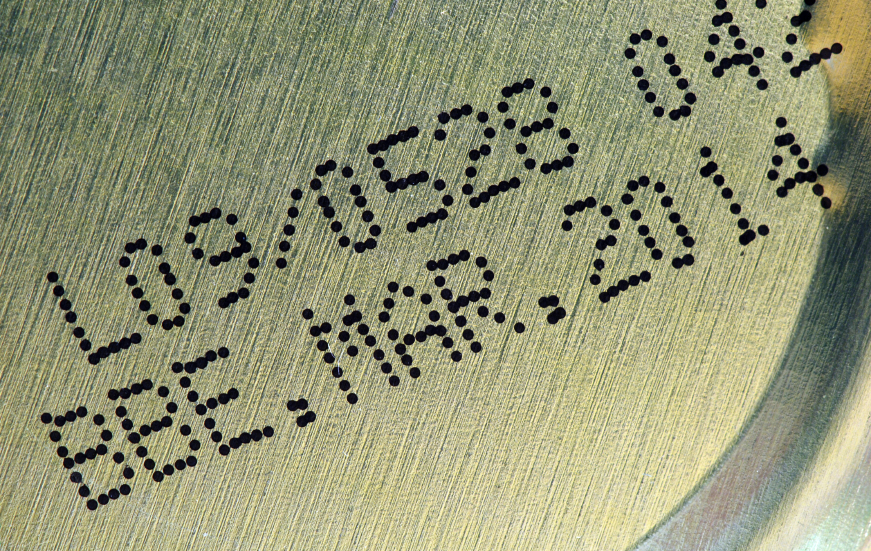
\includegraphics[width=0.60\textwidth]{images/bbdate222.jpg}
\end{figure}

This dissertation will be covering every aspect of this project including the following:
\newline 

- The Methodology of the project, the software development and research side of the project, the type of approach made to development, the testing of the project, the development tools used in this project such as GitHub and Visual Studio Code.
\newline

- The Technology Review, discussing the how and why the decision to create this application was made, why this is needed to help the workplace, is the project idea beneficial and sufficient, what a survey does to help with a project, the planning of the project basically the developer diary, technologies used in the project even extra ones if any, the references used in helping with the development of the software for the application, the issues and issues that arose during the software development, and the extras learned along the way.
\newline

- The System Design, how the application was designed and why, styling and HTML etc., design sketches for the application, what I wanted my application to do in terms of tackling the issue and any other extras added to the design element for example, making it easy for staff to use rather than making it complicated.
\newline

- The System Evaluation, the objectives and goals set out, were they achieved ?, the application testing results shown in a testing excel sheet, results of the conducted survey, and the limitations after the application was made.
\newline

- The Conclusion, where a look back at the rationale and goals of the overall project is done, highlighting the findings from the System Evaluation and discuss the opportunities and flexibility this project has made for me and for others especially the target audience, can it do more than one thing, can it benefit me for future interviews and possibly present this idea to potential investors etc.
\newline
\newpage
- The References and Appendices, this will include the GitHub repository for the software development of the application for the project and the references used to help develop the application and give a brief description for each reference. It will also include how to run the application accordingly. In this case it will contain the link for the Firebase website. Along with referenced URLs and technology used. It will also contain the project screen-cast presentation including a demonstration of the application.
\newline

- The Bibliography, includes any articles, pieces or reference to a quotation from it's citation. This is the information gained in the research on this particular field of product of date control in retail. Citations although little are spread out throughout the dissertation.

\begin{figure}[h!]
	\caption{GitHub Containing the Software Application for the Project.}
	\label{image:github}
	\centering
	
\includegraphics[width=0.7\textwidth]{images/github.png}
\end{figure}

This is the link to the GitHub Repository:
\newline
\url{https://github.com/AndreasFahey/AppliedProject-DateControl}
\newline

Here you will find all the project content both in software development, dissertation and any extras linked with the project.
You will also see issues raised during the project and if they were resolved. Also the commits and what was done for each commit will also be available to see the timeline in which things were done in the software development side of the project. This full dissertation will also be available on the GitHub repository as part of the download of the project along with a screen-cast, Power Point presentation, application testing results on a excel document and a screenshot of the results of the survey conducted put into a pie chart. 



